\documentclass[11pt, a4paper]{article}
\usepackage{pdfpages}
\usepackage{parallel}
\usepackage[T2A]{fontenc}
\usepackage{ucs}
\usepackage[utf8x]{inputenc}
\usepackage[polish,english,russian]{babel}
\usepackage{hyperref}
\usepackage{rotating}
\usepackage[inner=2cm,top=1.8cm,outer=2cm,bottom=2.3cm,nohead]{geometry}
\usepackage{listings}
\usepackage{graphicx}
\usepackage{wrapfig}
\usepackage{longtable}
\usepackage{indentfirst}
\usepackage{array}
\usepackage{tikzsymbols}
\usepackage{soul}
\usepackage[ruled,vlined]{algorithm2e}
%\counterwithout{figure}{section} 

\usepackage{url}
\makeatletter
\g@addto@macro{\UrlBreaks}{\UrlOrds}
\makeatother

\newcolumntype{P}[1]{>{\raggedright\arraybackslash}p{#1}}
\frenchspacing
\usepackage{fixltx2e} %text sub- and superscripts
\usepackage{icomma} % коскі ў матэматычным рэжыме
\PreloadUnicodePage{4}

\newcommand{\longpage}{\enlargethispage{\baselineskip}}
\newcommand{\shortpage}{\enlargethispage{-\baselineskip}}

\def\switchlang#1{\expandafter\csname switchlang#1\endcsname}
\def\switchlangbe{
\let\saverefname=\refname%
\def\refname{Літаратура}%
\def\figurename{Іл.}%
}
\def\switchlangen{
\let\saverefname=\refname%
\def\refname{References}%
\def\figurename{Fig.}%
}
\def\switchlangru{
\let\saverefname=\refname%
\let\savefigurename=\figurename%
\def\refname{Литература}%
\def\figurename{Рис.}%
}

\hyphenation{admi-ni-stra-tive}
\hyphenation{ex-pe-ri-ence}
\hyphenation{fle-xi-bi-li-ty}
\hyphenation{Py-thon}
\hyphenation{ma-the-ma-ti-cal}
\hyphenation{re-ported}
\hyphenation{imp-le-menta-tions}
\hyphenation{pro-vides}
\hyphenation{en-gi-neering}
\hyphenation{com-pa-ti-bi-li-ty}
\hyphenation{im-pos-sible}
\hyphenation{desk-top}
\hyphenation{elec-tro-nic}
\hyphenation{com-pa-ny}
\hyphenation{de-ve-lop-ment}
\hyphenation{de-ve-loping}
\hyphenation{de-ve-lop}
\hyphenation{da-ta-ba-se}
\hyphenation{plat-forms}
\hyphenation{or-ga-ni-za-tion}
\hyphenation{pro-gramming}
\hyphenation{in-stru-ments}
\hyphenation{Li-nux}
\hyphenation{sour-ce}
\hyphenation{en-vi-ron-ment}
\hyphenation{Te-le-pathy}
\hyphenation{Li-nux-ov-ka}
\hyphenation{Open-BSD}
\hyphenation{Free-BSD}
\hyphenation{men-ti-on-ed}
\hyphenation{app-li-ca-tion}

\def\progref!#1!{\texttt{#1}}
\renewcommand{\arraystretch}{2} %Іначай формулы ў матрыцы зліпаюцца з лініямі
\usepackage{array}

\def\interview #1 (#2), #3, #4, #5\par{

\section[#1, #3, #4]{#1 -- #3, #4}
\def\qname{LVEE}
\def\aname{#1}
\def\q ##1\par{{\noindent \bf \qname: ##1 }\par}
\def\a{{\noindent \bf \aname: } \def\qname{L}\def\aname{#2}}
}

\def\interview* #1 (#2), #3, #4, #5\par{

\section*{#1\\{\small\rm #3, #4. #5}}
\ifx\ParallelWhichBox\undefined%
    \addcontentsline{toc}{section}{#1, #3, #4}%
\else%
\ifnum\ParallelWhichBox=0%
    \addcontentsline{toc}{section}{#1, #3, #4}%
\fi\fi%

\def\qname{LVEE}
\def\aname{#1}
\def\q ##1\par{{\noindent \bf \qname: ##1 }\par}
\def\a{{\noindent \bf \aname: } \def\qname{L}\def\aname{#2}}
}

\newcommand{\interviewfooter}[1]{
\vskip 1em
\noindent \textit{#1}
}


\begin{document}

\title{1993 "--- Colani Mouse}
\date{}
\maketitle

По всей видимости, мышь Colani Mouse была, наравне с одноименным трекболом, первой среди так называемых <<дизайнерских>> манипуляторов, в разработке которых официально принимали участие звезды технического дизайна. Имя и форму данной мыши подарил Луиджи Колани (Luigi Colani) \cite{wiki}.

\textit{Наибольшую известность Колани получил в области автоиндустрии, отметившись четырьмя десятками концепт-каров; не менее активно он проектировал мебель, предметы домашнего обихода, бытовую технику. Плодотворное сотрудничество Луиджи Колани с немецкой компанией Vobis Microcomputer, владельцем торговой марки Highscreen, привело к выпуску на основе его дизайна нескольких персональных компьютеров, джойстиков, мышей и трекболов.}

\begin{figure}[h]
    \centering
    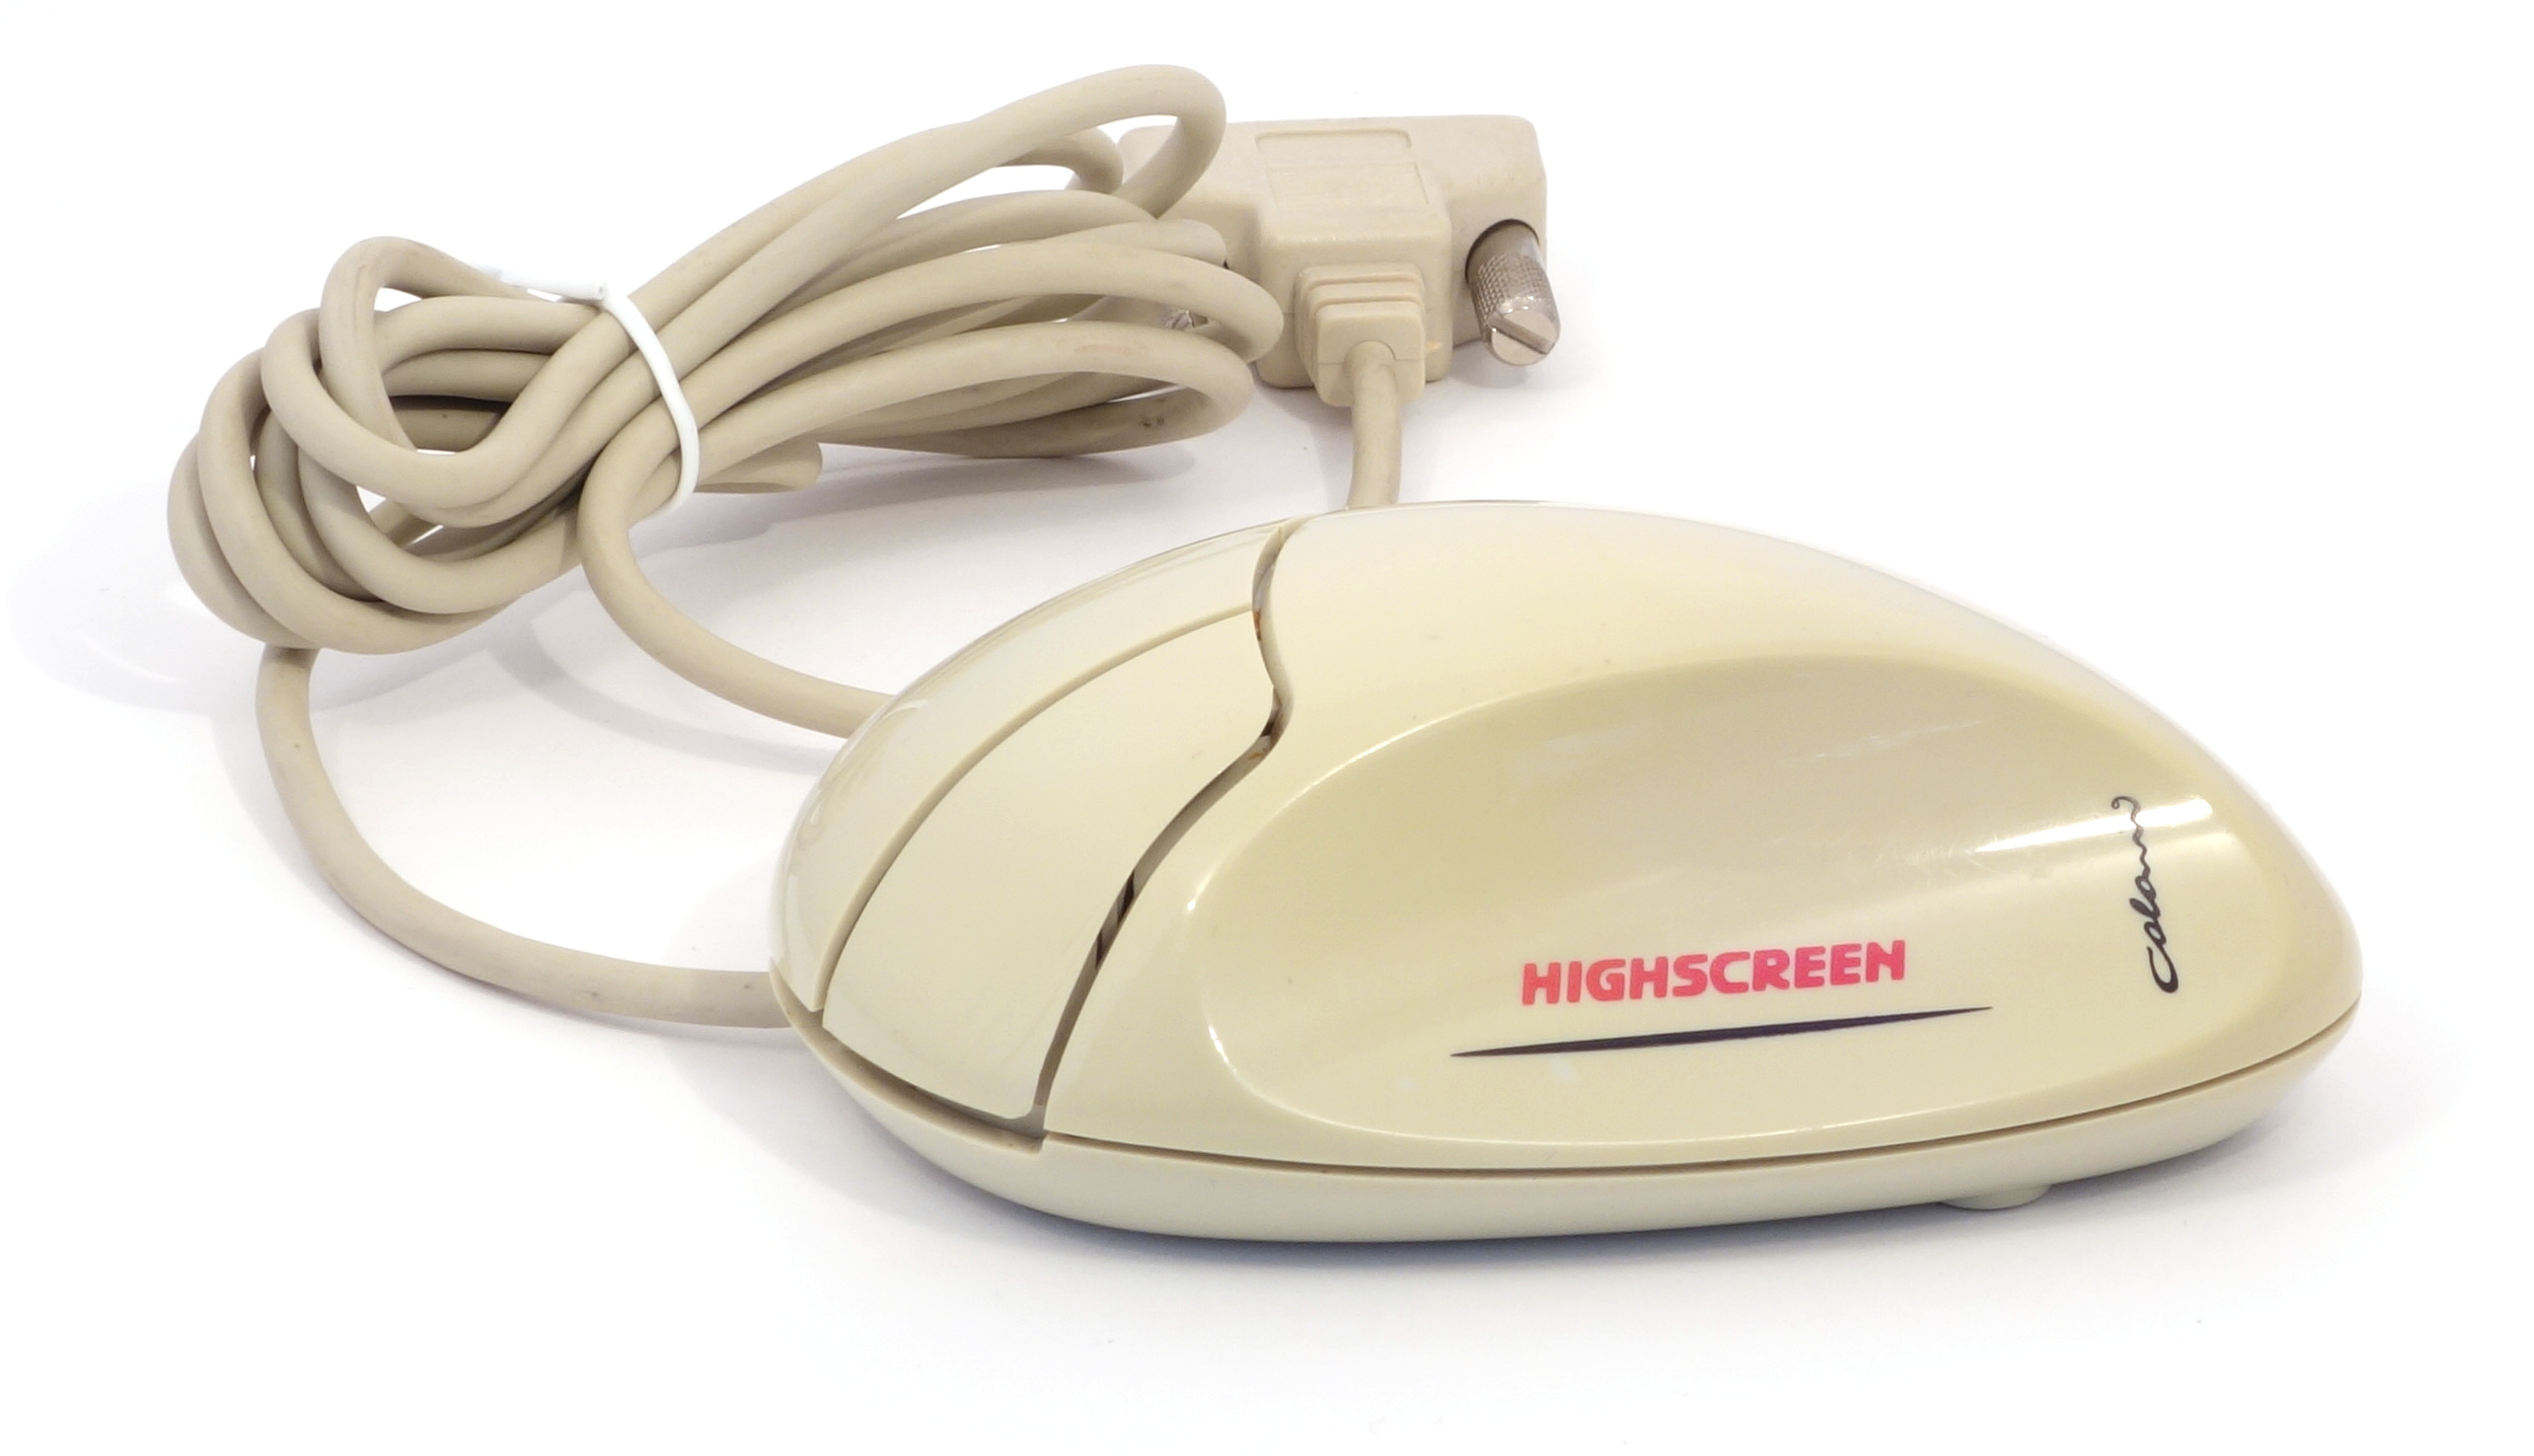
\includegraphics[scale=0.6]{1993_colani_mouse/pic_60.jpg}
    \caption{Colani Mouse}
    \label{fig:ColaniMousePic}
\end{figure}

Мышь HIGHSCREEN Colani Mouse, внешний вид которой показан на рис. \ref{fig:ColaniMousePic} "--- представитель этой линейки. Данная модель мыши (вместе с трекболом Colani Trackball того же производителя, имевшим сходный дизайн) выиграла престижную премию <<IF Design Award>> проектной организации «iF International Forum Design GmbH» в 1993 году \cite{award}.

\begin{figure}[h]
    \centering
    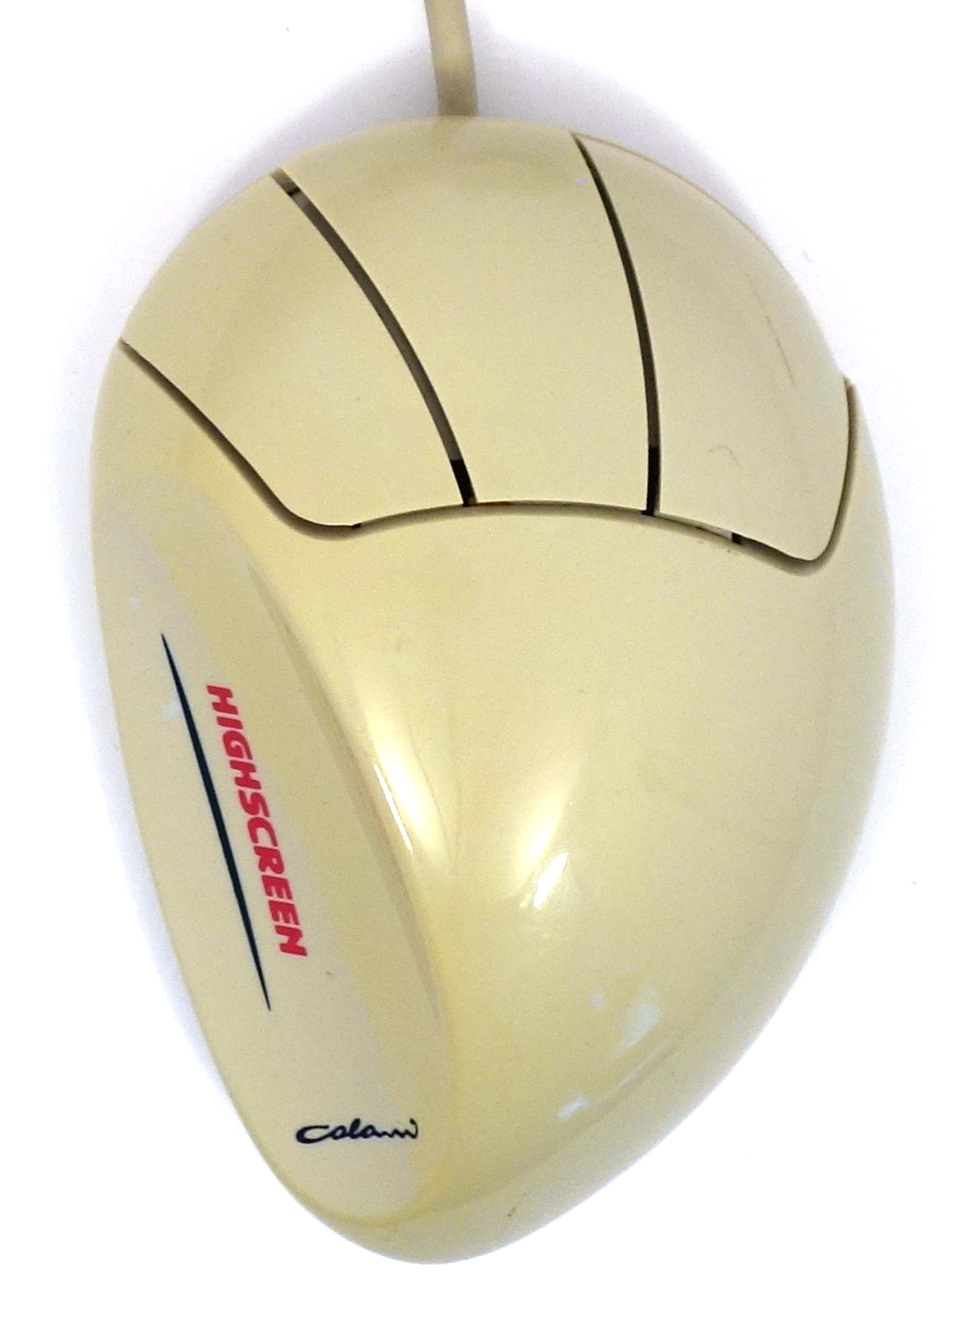
\includegraphics[scale=0.5]{1993_colani_mouse/top_60.jpg}
    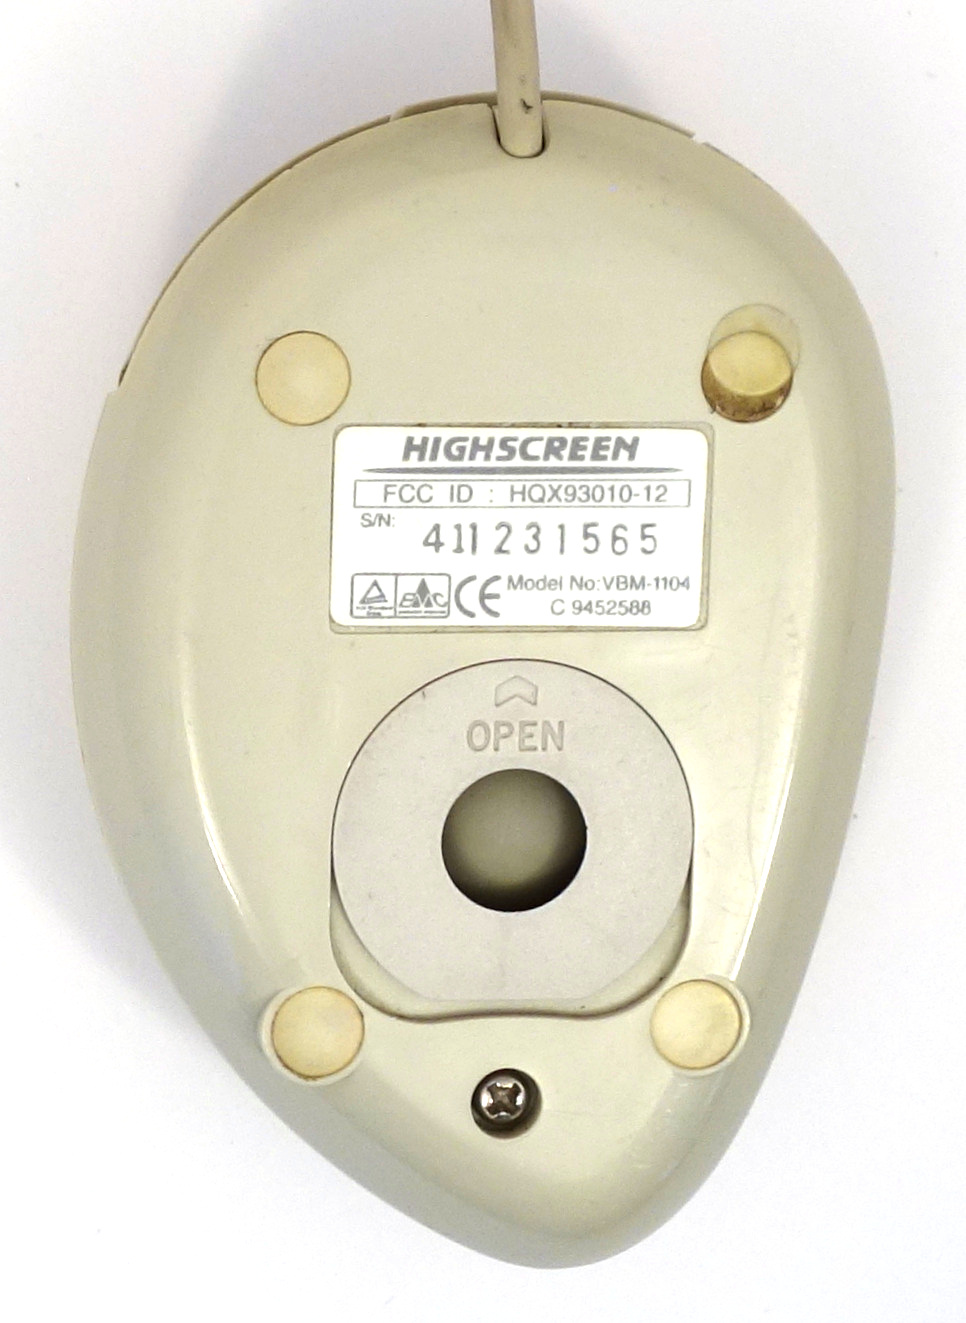
\includegraphics[scale=0.5]{1993_colani_mouse/bottom_30.jpg}
    \caption{Colani Mouse, вид сверху и снизу}
    \label{fig:ColaniMouseTopBottom}
\end{figure}

Начиная с концепт-каров, всячески подчеркивавших аэродинамику высоких скоростей, Луиджи Колани развил собственный новый стиль индустриального дизайна "--- бионику. Главный принцип бионики "--- придание предметам округлости и обтекаемых природных форм (рис. \ref{fig:ColaniMouseTopBottom}).

\textit{Как отмечают исследователи творчества Луиджи Колани, в целом дизайнер признавал первичность функции предмета перед его формой. Однако раз за разом он не мог устоять перед возможностью сделать изделие более <<природным>>, снабдить его изгибами, подчас сменяющими друг друга самым неожиданным образом, наводящим на мысли о скалах, подверженных длительной работе ветра или волн. В консервативных отраслях, например в автомобилестроении, такой подход обоснованно воспринимался как чересчур эксцентричный.}

Однако применительно к средствам управления курсором он оказался предвестником наступившей через некоторое время эры эргономичных мышей со сложной асимметричной формой, рассчитанной на максимально комфортное положение руки человека. Этой тенденции способствовало как то, что подобные формы легко воспроизводятся при литье пластиковых корпусов манипуляторов (чего нельзя сказать, например, о кузовах автомобилей), так и популярность глиняных моделей со следами сжимавшей их руки, позволявших разработчику без больших сложностей получить анатомически-точное и необычное внешне изделие. Впрочем, судя по некоторым признакам, сам Луиджи Колани не прибегал к такому способу получения формы.

Как можно видеть на рис. \ref{fig:ColaniMouseSize}, Colani Mouse является весьма компактным изделием, почти целиком помещающимся в ладони.

\begin{figure}[h]
    \centering
    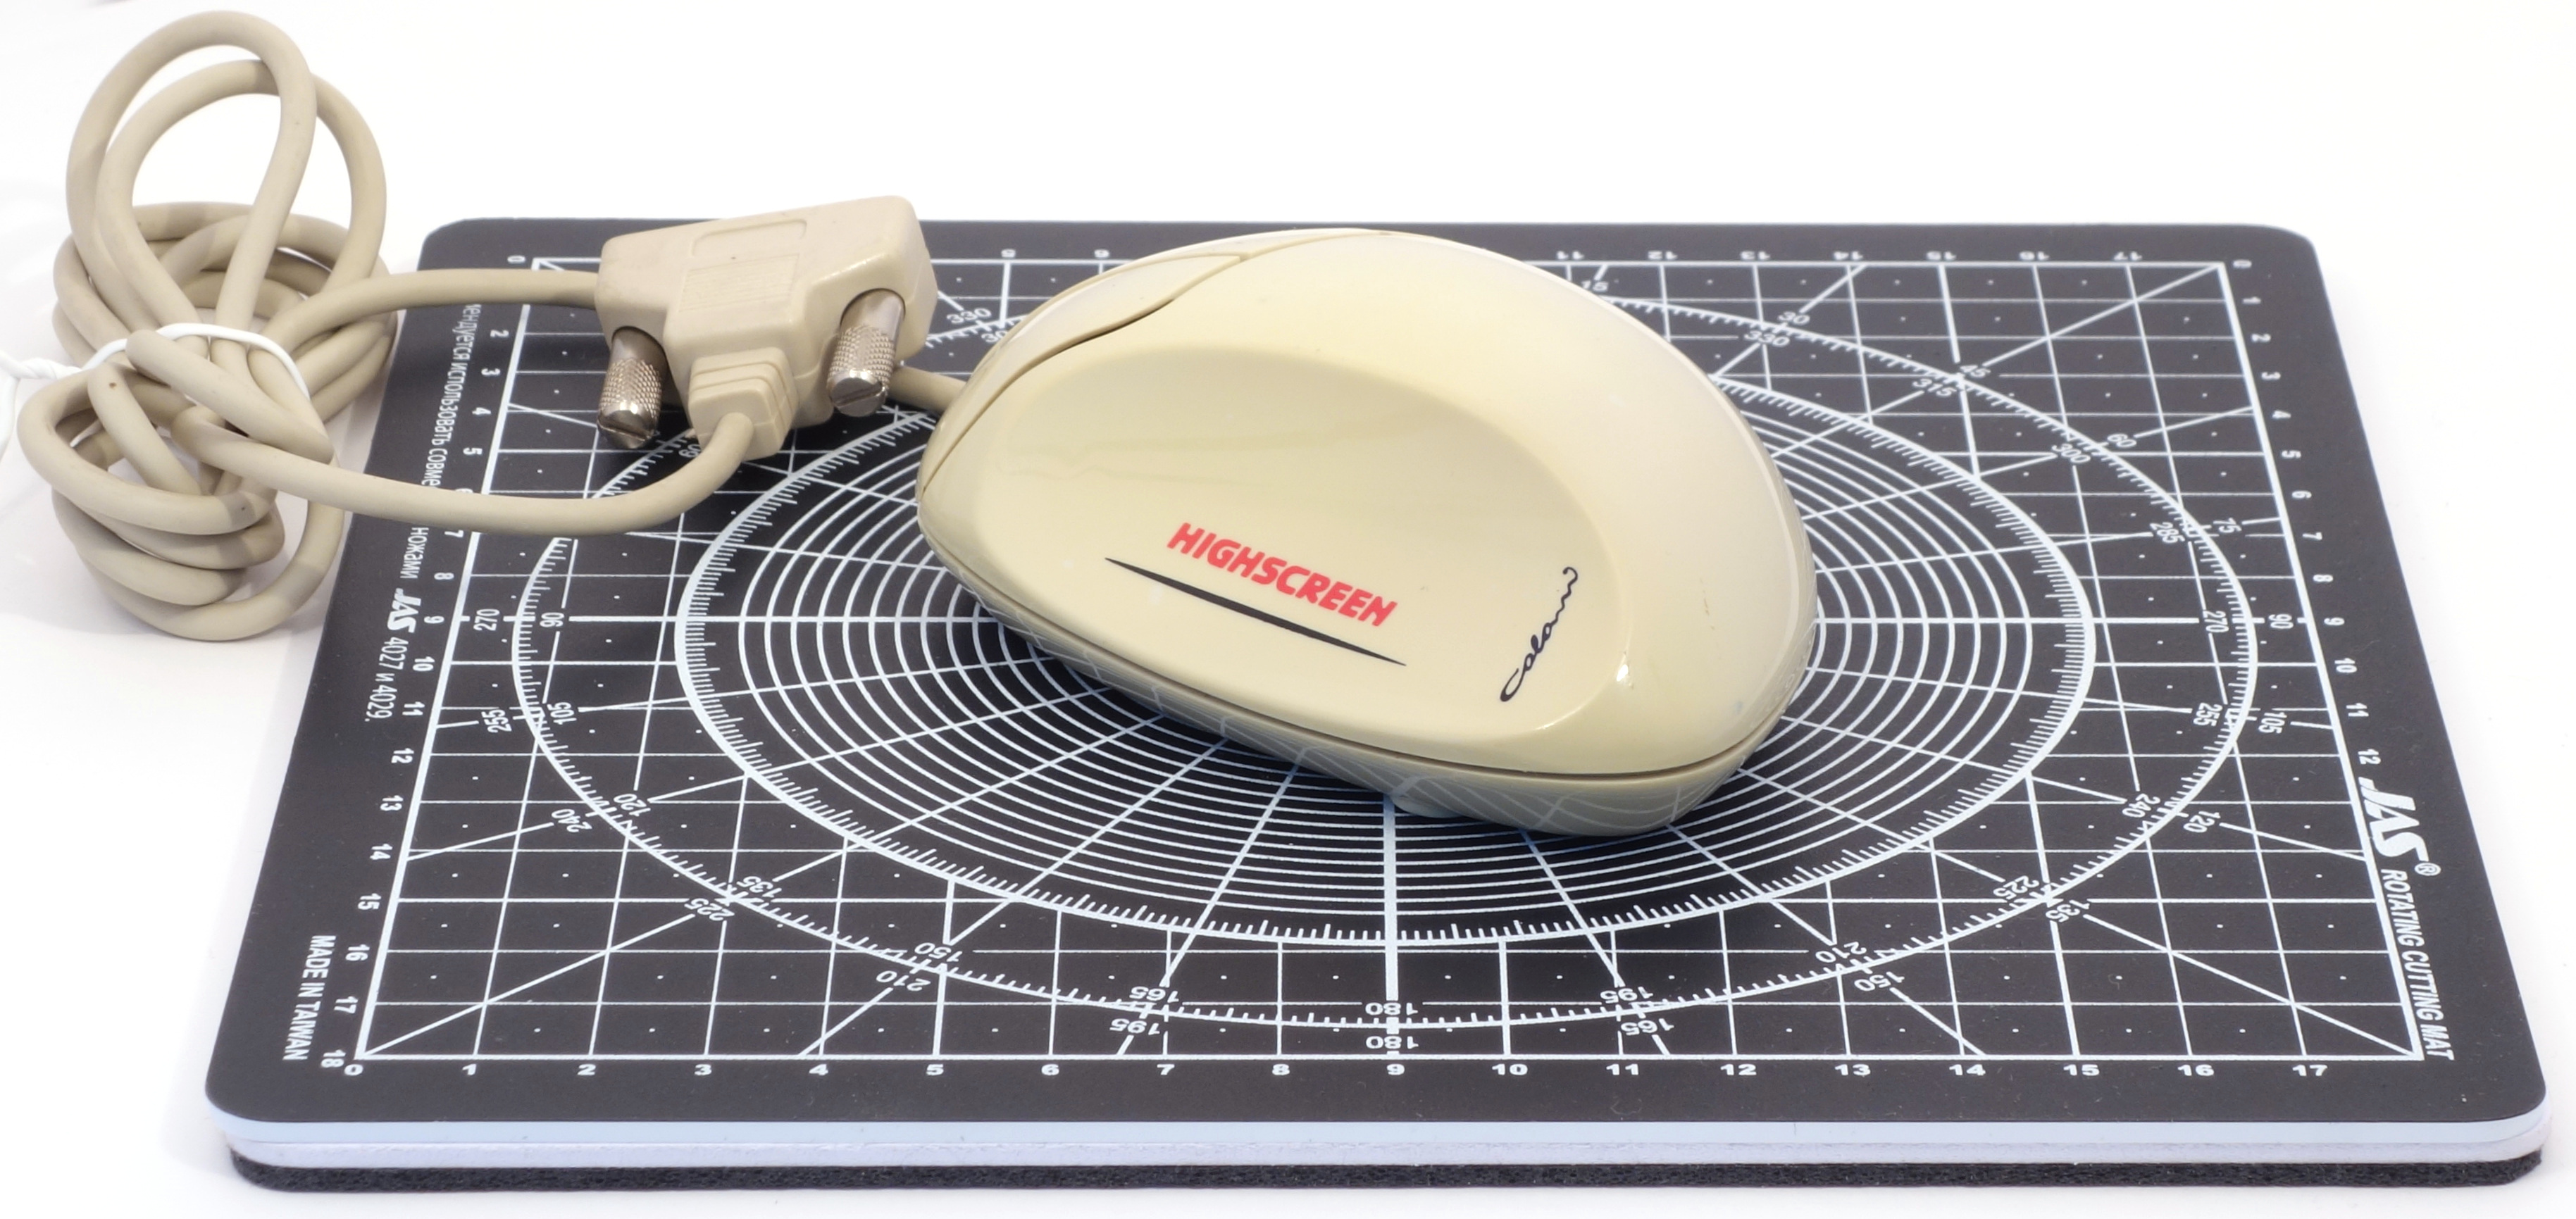
\includegraphics[scale=0.5]{1993_colani_mouse/size_30.jpg}
    \caption{Colani Mouse на размерном коврике с шагом сетки 1 см}
    \label{fig:ColaniMouseSize}
\end{figure}

Помимо того, что вогнутая часть корпуса несет эстетическую и художественную функцию, она служит опорой для большого пальца (рис. \ref{fig:ColaniMouseHand}). Однако на рис. \ref{fig:ColaniMouseSize} отчетливо видно, что данный элемент дизайна не доходит до конца корпуса, в результате чего образуется выступ, без которого держать мышь было бы однозначно комфортнее (эргономической курьезности этому выступу добавляет и то, он гордо подписан фамилией дизайнера). Кроме того, корпус не предоставляет пользователю опоры под запястье. Тем не менее, в целом положение руки на нем является удобным, клавиши расположены в хорошей доступности и имеют достаточную площадь.

\begin{figure}[h]
    \centering
    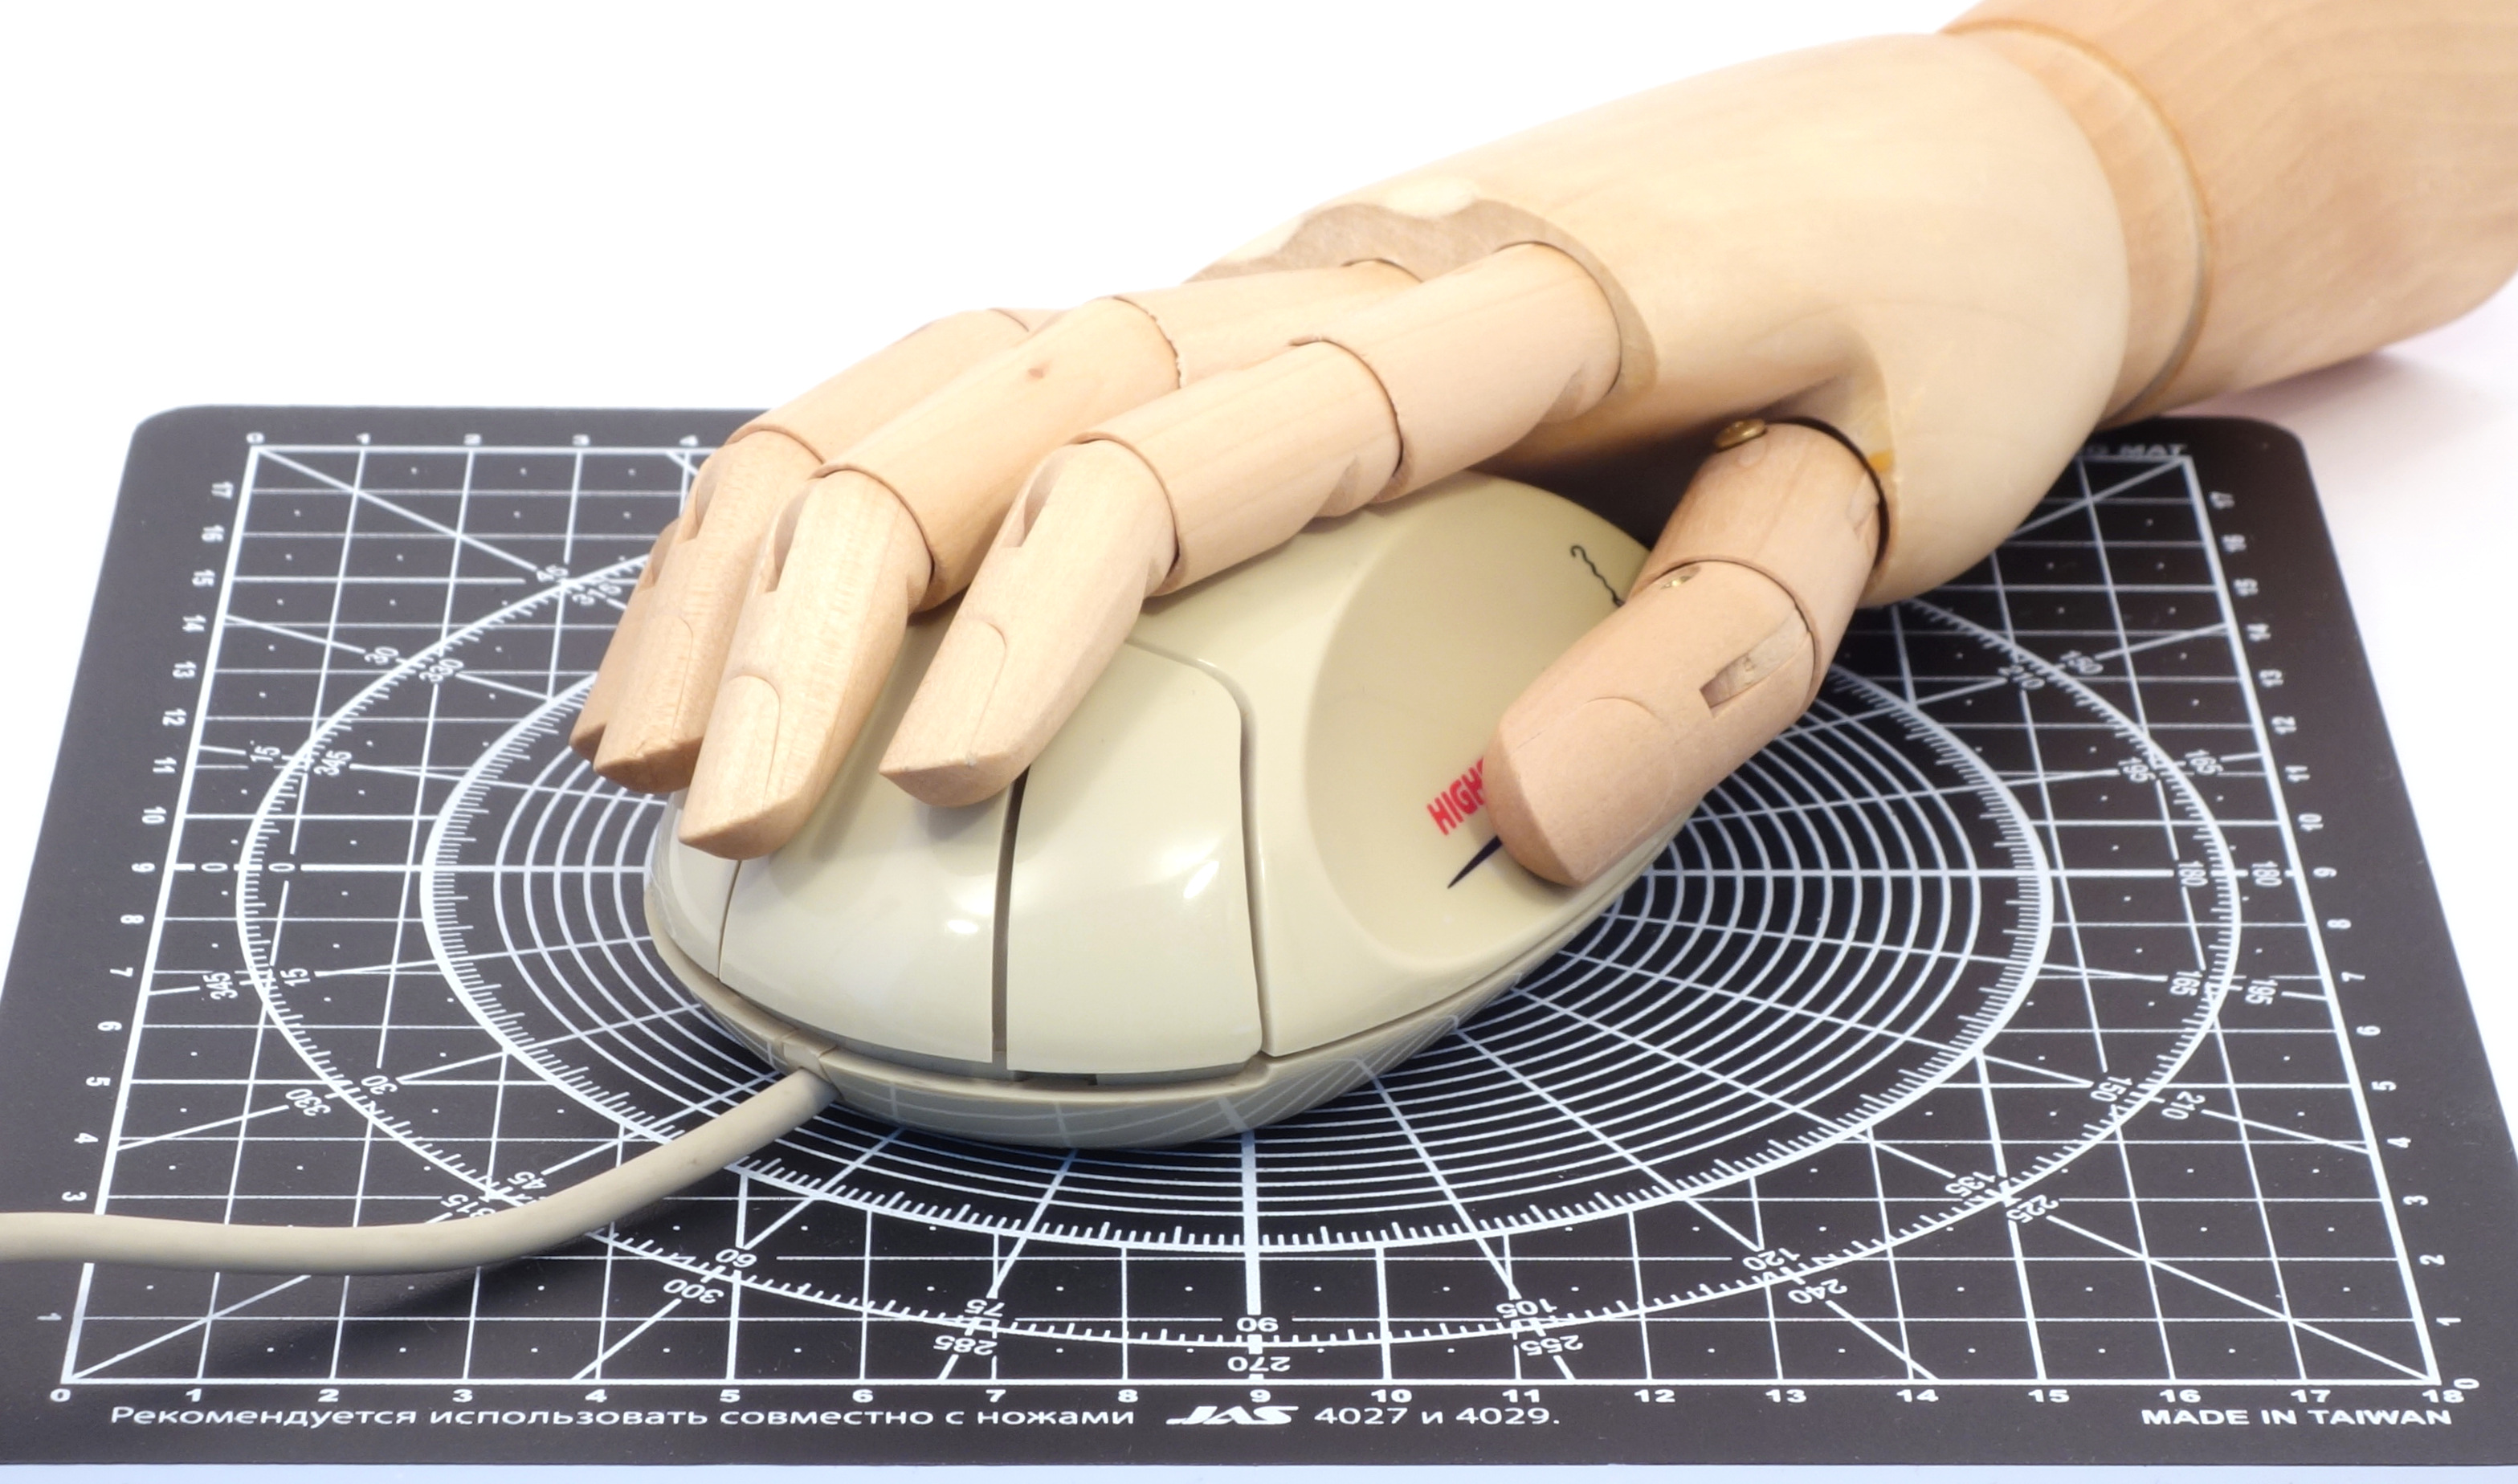
\includegraphics[scale=0.45]{1993_colani_mouse/hand_30.jpg}
    \caption{Colani Mouse в комплекте с моделью руки человека}
    \label{fig:ColaniMouseHand}
\end{figure}

Внутреннее устройство мыши, показанное на рис. \ref{fig:ColaniMouseInside}, позволяет классифицировать ее как оптомеханическую, с зубчатыми дисками энкодеров, характерными для конца 80-х "--- начала 90-х годов. Заметим, что выбор деталей является достаточно бюджетным: мышь содержит минимум металлических деталей. Также на рисунке можно заметить изоляционную ленту, скрывающую место сращивания кабеля: это очевидные последствия тенденции к повреждению изоляции кабеля в месте его выхода из корпуса "--- не самая редкая ситуация, когда в это месте конструкция мыши не  предусматривает гибкую предохранительную муфту.

\begin{figure}[h]
    \centering
    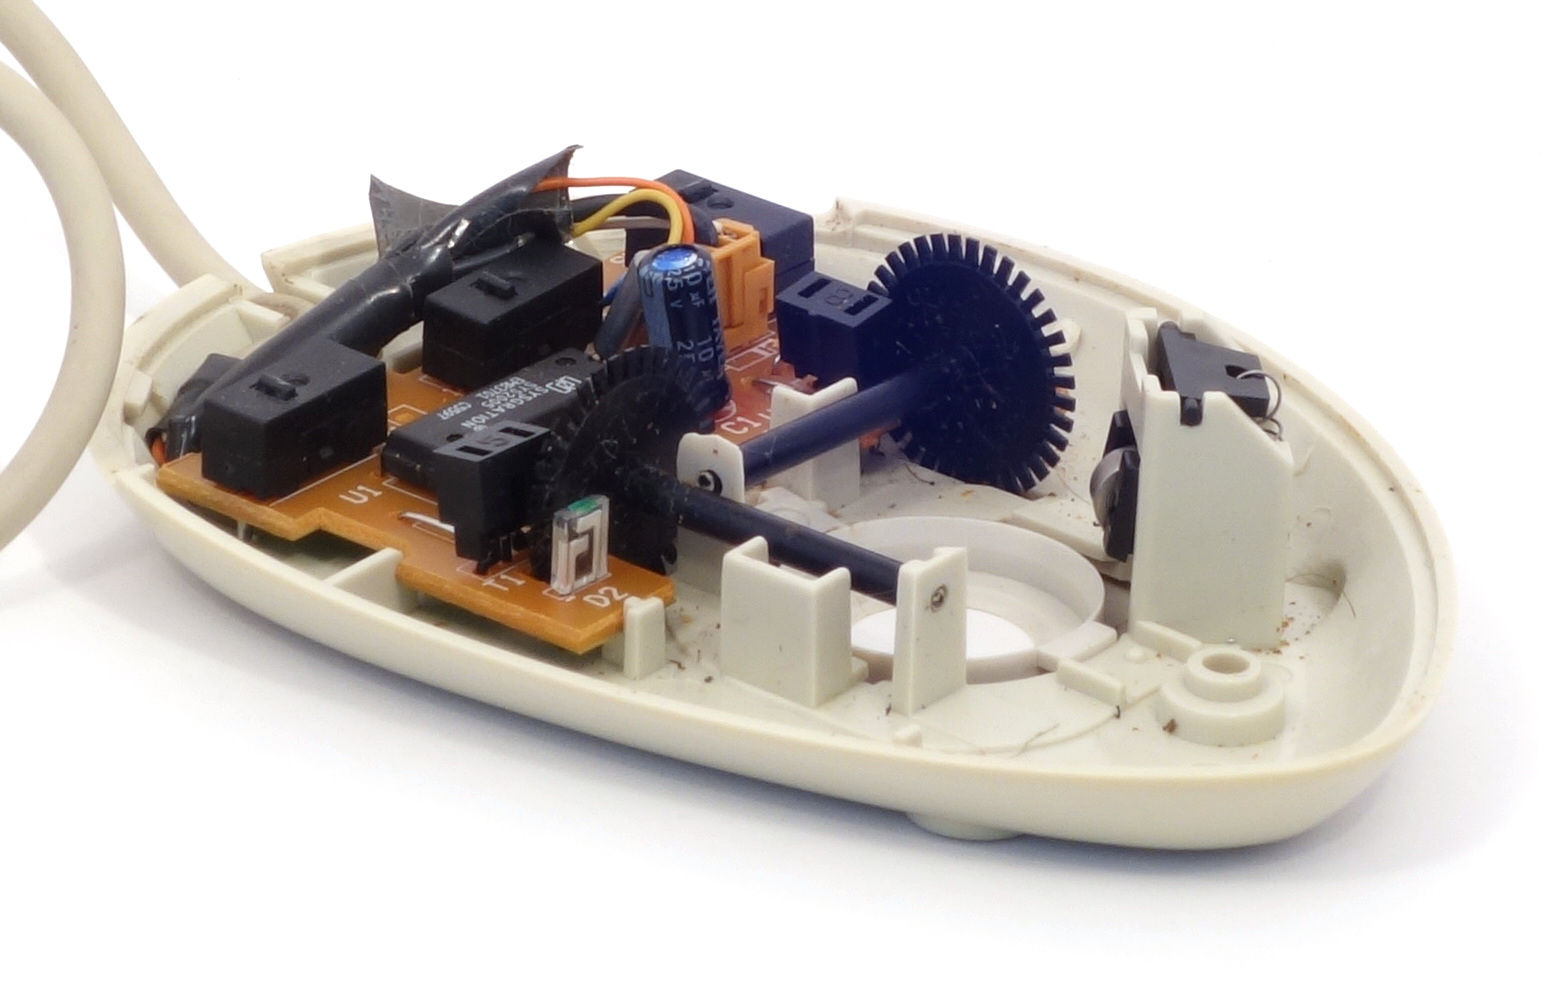
\includegraphics[scale=0.9]{1993_colani_mouse/inside_60.jpg}
    \caption{Colani Mouse в разобранном виде}
    \label{fig:ColaniMouseInside}
\end{figure}

\begin{thebibliography}{9}
    \bibitem {wiki} Luigi Colani – Wikipedia \url{https://en.wikipedia.org/wiki/Luigi_Colani}
    \bibitem {award} iF – HIGHSCREEN Colani Mouse \url{https://ifdesign.com/en/winner-ranking/project/highscreen-colani-mouse/19312}
\end{thebibliography}

\end{document}
